\chapter*{Introduction}
\label{ch:Introduction}
This report illustrates development and findings of Group 2's project for
the course Text Analytics, Academic Year 2024-2025.

% \section*{Team members and roles}


% copy-pasted from project proposal
\section*{Motivation and project goal}
% Songs have the unique ability to engage people in ways that few other
% mediums can match. While beats and melodies contribute to this impact,
% it is often the lyrics that give songs their true emotional strength.
% Lyrics serve as one of the main foundations of songs, playing
% a crucial role in expressing feelings in many different ways.
% Analyzing the emotional tone of song texts can give useful insights about individual mental states,
% cultural trends, social issues and more.\\
% The main goal of this project is to perform emotion detection on stanzas of songs.
This project's goal is the development of various Machine Learning models that perform 
emotion detection on songs' lyrics.\\
The emotional tone of songs can be useful
for many things, such as automatized playlist creation, or songs' organization,
offering an alternative to the more traditional genre-based classification.\\
To obtain a deeper understanding of
emotional fluctuations within the texts,
the models assign emotion labels
to individual stanzas instead of full songs.
The emotional classification is based on Robert Plutchik's eight primary emotions
(shown in figure~\ref{fig:primary_emotions}),
offering a comprehensive range for representing diverse emotional states.\\
\begin{figure}[H]
    \centering
    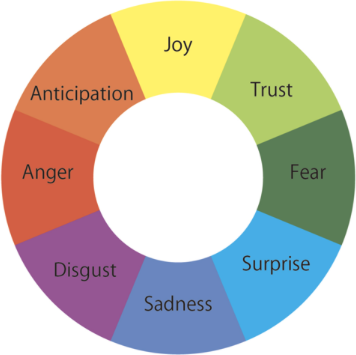
\includegraphics[scale= 0.5]{pictures/plutchik_primary_emotions.png}
    \caption{Plutchik's eight primary emotions}
    \label{fig:primary_emotions}
\end{figure}


% Furthermore, we intend to compare different textual preprocessing and
% Machine Learning models, in order to explore different possibilities and
% evaluate their performances.


\section*{Dataset overview}
The dataset used in this project represents a sampled subset of songs
derived from the Genius Song Lyrics Dataset\textsuperscript{\cite{geniusdataset}}.
The original dataset (3m records) included songs in many different languages; however, this work focused
exclusively on English-language songs.
The original dataset contained numerous attributes, but the ones considered relevant
for model training are:

\begin{itemize}
    \item \textbf{title:} the song's title;
    % \item \textbf{artist:} the artist
    % \item \textbf{year:}
    % \item \textbf{views:}
    % \item \textbf{features:}

    % \item \textbf{id:}
    \item \textbf{lemmatized\_stanzas:} lyrics of the single stanza;
    
    \item \textbf{stanza\_number:} identifies the position of the stanza in the song;

    \item \textbf{is\_chorus:} boolean variable that attests whether the stanza is
        a chorus;
    
    \item \textbf{tag:} represents the genre of the song. for easier handling,
        it is split into boolean attributes
        (is\_country, is\_pop, is\_rap, is\_rb, is\_rock);

    \item \textbf{label:} represents the emotional classification of the stanza,
        assigned by Albert Base v2\textsuperscript{\cite{albert-base-v2}} model.
    
    % \item \textbf{is\_country:}
    % \item \textbf{is\_pop:}
    % \item \textbf{is\_rap:}
    % \item \textbf{is\_rb:}
    % \item \textbf{is\_rock:}
\end{itemize}

% The dataset originally didn't contain emotion labels, essential for training the models.
% To create the ground truth, the model
% Albert Base v2\textsuperscript{\cite{albert-base-v2}} was used, classifying
% stanzas' lyrics into Plutchik's eight primary emotions.
Due to limited computational power, the labeling process was time-intensive,
ultimately resulting in a limited dataset \textbf{(QUANTE? AGGIUNGEREI NUMERO STROFE)}.\\